\documentclass{article}
\usepackage{ctex}
\usepackage{fontspec}
\usepackage{listings}
\usepackage{xcolor}
\usepackage{geometry}
\usepackage{graphicx}
\usepackage{float}
\usepackage{amsmath}
\usepackage{minted}
\usepackage{tabularx}
\usepackage{makecell}
\usepackage{array}
\usepackage{booktabs}
\usepackage{algorithm2e}
\geometry{a4paper,scale=0.8}
\definecolor{codebg}{rgb}{0.95,0.95,0.95}
\begin{document}
\title{\Huge \centering \textbf{基于词频-逆词频分析($TF-IDF$)的新闻文本分类器}}
\date{}
\maketitle
\setlength{\parskip}{0.5\baselineskip}
\section*{\LARGE 一、导言}
近年来,随着互联网的快速发展,大量的新闻文章每天在网络上涌现出来。对于用户而言,如何快速准确地获取感兴趣的新闻信息成为一项具有挑战性的任务。而对于新闻提供方而言,如何对新闻进行自动分类,则可以提高其新闻发布的效率和用户体验。

新闻文本分类任务是自然语言处理领域的重要问题之一。它旨在将一篇给定的新闻文本自动分类到预定义的类别中,如体育、政治、娱乐等。传统的文本分类方法主要依赖于手工构建的特征和规则,但这些方法存在特征提取难、规则设计繁琐等问题。近年来,基于机器学习的方法在新闻文本分类任务中取得了巨大的成功。

本实验报告的主要目标是通过使用$TF-IDF(term\ frequency-inverse\ document\ frequency)$特征表示和逻辑斯蒂回归$(Logistic\ Regression)$,对新闻文本进行自动分类。tf-idf是一种常用的文本特征表示方法,它通过统计单词在文本中的词频和逆文档频率来反映其在整个语料库中的重要程度。SVM是一种常用的分类算法,它通过在高维空间中构造一个最优的超平面来实现分类的目的。

通过本实验的研究,我们期望能够探索和验证$TF-IDF$方法在新闻文本分类任务中的有效性和性能。这将有助于提高自动化新闻分类系统的准确性和效率,为用户提供更好的新闻浏览体验。

\section*{\LARGE 二、解决方法}
\subsection*{\Large 1、问题定义}
给定语料$\mathcal{C}=\{t_1,t_2,\dots,t_n\}$,其中$t_i,\ i=1,2,\dots,$为单字,每个语料$C_i$对应一个离散的标签$y_i=enumerate(1,2,\dots)$。根据语料的字特征,找到一个映射$\mathcal{F}$,使得$\mathcal{F}(C_i)=y_i$,


\subsection*{\Large 2、问题的解决与推导}

在本实验中,我们使用了$TF-IDF$方法对新闻文本进行分类。$TF-IDF$方法是一种常见的文本信息处理方法,广泛运用于自然语言处理的统计学习中。它结合了词频和逆文档频率两个因素,对文本进行权重计算,以便更好地表示文本的特征。

这里我们可以使用以下公式来计算文本中每个词汇的$TF-IDF$值:

\begin{equation}
\text{TF-IDF}(t,d) = \text{TF}(t,d) \times \text{IDF}(t)
\end{equation}

其中,$\text{TF}(t,d)=\cfrac{N_t}{N}$表示词汇$t$在文本$d$中的词频,这里的$N_t$表示词汇$t$在文中出现的次数,$N$表示文章的总词数。$\text{IDF}(t)$则表示词汇$t$的逆文档频率。逆文档频率可以使用以下公式来进行计算:

\begin{equation}
\text{IDF}(t) = \log\frac{N}{n_t}
\end{equation}
其中,$N$表示文档总数,$n_t$表示包含词汇$t$的文档数。

从公式中可以看出,$TF-IDF$值高的词汇在文本中出现频率高,但在整个文集中出现频率相对较低。这说明对于某一个文章里面的某一个词来说,如果这个词的$TF-IDF$值越高,
那么它就越具有代表性,因此,$TF-IDF$值可以很好地表示文本中的重点词汇,从而进行文本分类和信息检索。

对于本次实验的新闻文本分类任务来说,我们可以使用$TF-IDF$来分析不同文章中最具有代表性的词,通过这些典型意义词的分析,可以实验对不同类型的新闻进行自动分类。

完成$TF-IDF$的关键词向量提取之后,我们使用逻辑斯蒂回归$(Logistic\ Regression)$算法对$TF-IDF$向量进行分类。在逻辑斯蒂回归中,我们使用逻辑斯蒂函数对数据进行建模和预测。逻辑斯蒂函数可以将输入值在$0$和$1$之间进行映射,表示该样本属于某一类别的概率。逻辑斯蒂函数的公式如下:

\begin{equation}
h_{\theta}(x)=\frac{1}{1+e^{-\theta^Tx}}
\end{equation}

其中,$h_\theta(x)$表示某个样本$x$属于某一类别的概率,$\theta$表示要学习的参数,$e$表示自然常数。我们可以通过最大化似然函数 $L(\theta)$ 来学习模型参数:

\begin{equation}
L(\theta)=\prod_{i=1}^{m}h_{\theta}(x^{(i)})^{y_i}(1-h_{\theta}(x^{(i)}))^{1-y_i}
\end{equation}

其中,$y_i$表示样本$x^{(i)}$的类别标签,$m$表示样本总数。我们需要最大化似然函数以求得最优的 $\theta$ 参数值,可以通过梯度下降法等不同的数值优化方法进行优化。
不过在训练的过程中,我们通常会为这个训练函数添加一个正则项以保证参数能够更好收敛于一个较小的数值内,即优化函数应该为
\begin{equation}
    \hat{L}(\theta)=\prod_{i=1}^{m}h_{\theta}(x^{(i)})^{y_i}(1-h_{\theta}(x^{(i)}))^{1-y_i}+\frac{1}{2}C\sum_{j=1}^{m}\theta_j^2
\end{equation}
这里我们使用的是$L2$正则项。

使用逻辑斯蒂回归进行分类时,我们可以通过将逻辑斯蒂函数的输出值大于$0.5$的样本归为一类,小于$0.5$的归为另一类。同时,逻辑斯蒂回归也可以输出概率值,在进行一些特殊的数据处理或者评估时非常有用。

除去$TF-IDF$方法之外,常见的方法还包括词向量分析以及深度学习等方法,词向量分析目前主流的方法是$word2vec$模型训练,但是使用这种方法不可避免会导致模型误分析许多无关信息,模型本身并不具备判断哪些
信息是关键并且重要的。故虽然词向量在含义表达上有着非常强大的能力,仅靠词向量本身分析的效果却并不能取得非常好的效果。另一方面,深度学习的方法训练成本较高,包括时间与金钱上的成本。值得一提的是,深度
学习的方法往往与词向量法结合起来使用,不过目前神经网络的许多现象仍然具有不可解释性,相比机器学习方法在模型的调整上有着更高的难度。

相比之下,$TF-IDF$简单有效,并且在大语料数据集中有着非常好的特征抽取能力。

\begin{algorithm}[H]
    \SetAlgoLined
    \KwIn{语料$\mathcal{C}$, 词汇集合$\mathcal{T}=\{t_1,t_2,\dots\}$}
    \KwOut{$TF-IDF$矩阵}
    计算每个单词在每篇文档中的词频$TF$:\\
    \ForEach{文章$c_j\in \mathcal{C}$}{
        \ForEach{词汇$t_i\in \mathcal{T}$}{
            计算单词$t_i$在文档$c_j$中的词频tf:\\
            $TF(t_i, c_j) = \cfrac{n_{ti}}{N_j}$
        }
    }
    
    计算每个单词在语料集合$\mathcal{C}$中的逆文档频率$IDF$:\\
    \ForEach{词汇$t_i\in \mathcal{T}$}{
        统计含有单词$t_i$的文档数量$doc\_count$\\
        计算单词w的逆文档频率$IDF$:\\
        $IDF(t_i) = log\cfrac{|\mathcal{C}|}{doc\_count + 1}$
    }
    
    计算每个单词在每篇文档中的$TF-IDF$值:\\
    \ForEach{文档$C_j \in \mathcal{C}$}{
        \ForEach{词汇$t_i\in \mathcal{T}$}{
            计算单词$t_i$在文档$C_j$中的$TF-IDF$值:\\
            $TF-IDF(t_i, C_j) = TF(w, d) * IDF(w)$
        }
    }
    
    \caption{$TF-IDF$算法流程}
\end{algorithm}
\section*{\LARGE 三、实验}
实验所使用的数据集来自阿里云天池“零基础入门NLP - 新闻文本分类”比赛,实验所使用的为中文脱敏语料,原始文字数据均通过某个字典
进行了加密。

\begin{tabular}{|p{2cm}|p{13cm}|} 
    \hline
    $tag$ & $data$ \\
    \hline
    $6$ & $57\ 44\ 66\ 56\ 2\ 3\ 3\ 37\ 5\ 41\ 9\ 57\ 44\ 47\ 45\ 33\ 13\ 63\ 58\ 31\ 17\ 47\ 0\ 1\ 1 \dots $\\
    \hline
 \end{tabular}

 这里$data$中每个字都用一个特定的$id$表示。
 
 从上文的算法流程图可以看出,由于$TF-IDF$本身输入只有语料$\mathcal{C}$和词汇集$\mathcal{T}$,并没有显式的训练过程,整个流程其实
 是计算一个$TF-IDF$矩阵,并由该矩阵推得结果,这一部分并不需要设置任何参数。

 \subsection*{1、实验结果}
 逻辑斯蒂回归分类部分需要设置超参数$C$,以确定正则化强度。实验中我们取$C=4.0$。从$200000$条测试数据抽取$10\%$作为测试数据,最终得到的$ROC$曲线:
 \begin{figure}[H]
    \centering
    \begin{minipage}[t]{1.0\linewidth}
        \centering
        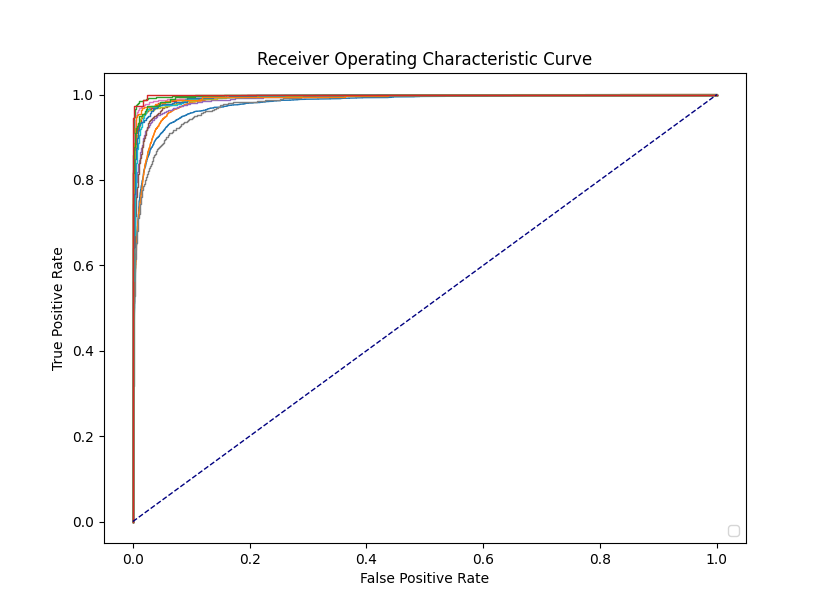
\includegraphics[height=10cm]{Figure_1.png}
        \caption{模型预测的$ROC$曲线}
    \end{minipage}
 \end{figure}
 图中不同颜色的曲线表示模型对不同类别的二分类$ROC$曲线。可以看到模型的预测结果非常理想。
 \begin{figure}[H]
    \centering
    \begin{minipage}[t]{1.0\linewidth}
        \centering
        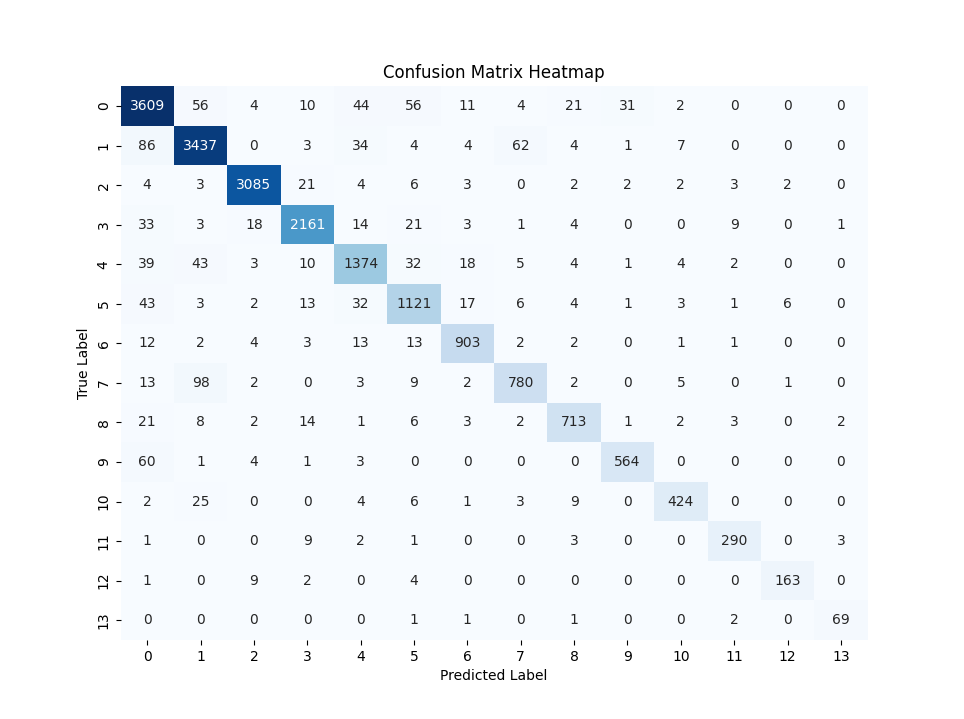
\includegraphics[height=10cm]{Figure_2.png}
        \caption{模型预测的混淆矩阵热力图}
    \end{minipage}
 \end{figure}
 实验报告的总准确率
 \begin{minted}[linenos,breaklines,bgcolor=codebg]{python3}
    训练集准确率: 0.9488611111111112 
    测试集F1 Score: 0.9251220754849809
 \end{minted}
这里$F1\ Score$的计算公式
$$F1\ Score=\cfrac{2\times precision \times recall}{precision+recall}$$
\subsection*{\Large 3、实验关键代码}
\noindent 实验所用模块
\begin{minted}[linenos,breaklines,bgcolor=codebg]{python3}
from gensim import models
import pandas as pd
from sklearn.linear_model import LogisticRegression
from sklearn.feature_extraction.text import TfidfVectorizer
from sklearn.model_selection import train_test_split
from sklearn.metrics import accuracy_score, precision_score, recall_score, f1_score, confusion_matrix,roc_curve
import seaborn as sns
import numpy as np
import matplotlib.pyplot as plt
\end{minted}
数据的读取以及预处理
\begin{minted}[linenos,breaklines,bgcolor=codebg]{python3}
train_df = pd.read_csv('train_set.csv', sep='\t')
train_tag=train_df['label']
train_rawdata=[data for idx,data in enumerate(train_df['text'])]
train_data=[data.split(' ') for idx,data in enumerate(train_df.iloc[:,1])]

test_df = pd.read_csv('test_a.csv', sep='\t')

test_rawdata=[data for idx,data in enumerate(test_df['text'])]
test_data=[data.split(' ') for idx,data in enumerate(test_df.iloc[:])]

try:
    word2vec_model=models.Word2Vec.load('word2vec.model')
    print('load complete')
except:
    print('no model')
    word2vec_model=models.Word2Vec(sentences=train_data+test_data, vector_size=100,workers=4)
    word2vec_model.save('word2vec.model')

\end{minted}
数据的训练以及可视化
\begin{minted}[linenos,breaklines,bgcolor=codebg]{python3}
word_vectorizer=TfidfVectorizer(sublinear_tf=True,
strip_accents='unicode',
analyzer='word',
token_pattern=r'\w{1,}',
stop_words='english',
ngram_range=(1, 1),
max_features=10000,
)
word_vectorizer.fit(train_rawdata+test_rawdata)
train_word_features = word_vectorizer.transform(train_rawdata)
test_word_features = word_vectorizer.transform(test_rawdata)

X_train = train_word_features
y_train = train_tag
x_train_, x_valid_, y_train_, y_valid_ = train_test_split(X_train, y_train, test_size=0.1)

classifier=LogisticRegression(C=5)
classifier.fit(x_train_,y_train_)

y_pred = classifier.predict(x_valid_)
y_score=classifier.decision_function(x_valid_)
train_scores = classifier.score(x_train_, y_train_)
print(train_scores, f1_score(y_pred, y_valid_, average='macro'))
for i in range(14):
    fpr,tpr,_=roc_curve(y_valid_,y_score[:,i],pos_label=i)
    plt.plot(fpr, tpr,  lw=1)

plt.plot([0, 1], [0, 1], color='navy', lw=1, linestyle='--')
plt.xlabel('False Positive Rate')
plt.ylabel('True Positive Rate')
plt.title('Receiver Operating Characteristic Curve')
plt.legend(loc="lower right")
plt.show()

cm = confusion_matrix(y_valid_, y_pred)

sns.heatmap(cm, annot=True, cmap='Blues', fmt='g', cbar=False)
plt.title('Confusion Matrix Heatmap')
plt.xlabel('Predicted Label')
plt.ylabel('True Label')
plt.show()
\end{minted}
\section*{\LARGE 四、结论}
利用$TF-IDF$以及逻辑斯蒂回归的方式,本文成功完成了对脱敏新闻文本分类的任务,相比于其他方法如词向量分析等,$TF-IDF$有着
非常强大的特征提取能力,特别是对于关键以及典型特征分析有着非常健壮的性能。并且由于是基于统计学习的方法,并不需要深度学习的庞大
模型数据以及冗长的训练过程,简单快速,原理清晰。

总之,基于$TF-IDF$和逻辑斯蒂回归的模型在中长篇的新闻文本分类的任务中有着非常好的性能表现。不过值得注意的是,由于$TF-IDF$矩阵是通过
大量的数据得到的,使用$TF-IDF$分析法时必须要保证数据规模充分,否则可能会导致结果变差。
\end{document}  